\documentclass{beamer}
\usepackage[utf8]{inputenc}
\usepackage[romanian]{babel}
\usepackage{hyperref}
\usepackage{mathtools}
\usepackage{listings}
\usepackage{graphicx}
\usepackage{float}
\usepackage{xcolor}
\usepackage{adjustbox}
\usepackage{scalerel}
\usepackage{tikz}
\usetikzlibrary{arrows}
\usetikzlibrary{calc}
\usepackage{pgfplots}

\setbeamercovered{transparent}
\usetheme{Madrid}
\title{Traffic Manager}
\author{Student: Mihai Andrei Gherghinescu \\ Supervizor: Lect. Dr. Todor Ivașcu}

\graphicspath{ {./images/} }

\begin{document}

\frame{\titlepage}

\section{Introducere}
    \begin{frame}{Introducere}
        Una dintre principalele cauze ale congestiilor in trafic
        sunt intersectiile. Acest fenomen este in special observat in 
        zonele urbane unde prezenta acestora este abundenta. 
        Pentru a minimiza timpul pierdut atat cat si siguranta soferilor 
        au fost dezvoltate sisteme de trafic inteligente(ITS). Acest 
        concept a fost reinventat dealungul timpului iar in prezent 
        este cuprins in notiunea de "smart city". Urmeaza sa prezint un 
        scurt istoric al evolutiei ITS cat si sa 
        prezint contributia proprie prin prezentarea unui nou tip de sistem.
    \end{frame}

\section{Privire de ansamblu asupra tehnologiei dezvoltate}
    \begin{frame}{Privire de ansamblu asupra tehnologiei dezvoltate}
        Dealungul timpului au fost concepute numeroase abordari ale 
        gestionari traficului. Noi o sa prezentam unele dintre cele 
        mai recente abordari care au dovenit a aduce imbunatatiri asupra
        traficului:
        \begin{itemize}[<+-| alert@+>]
            \item Sisteme bazate pe detectia de obiecte 
            \item Sisteme bazate pe senzori
            \item Sisteme care sincronizeaza traficul
            \item Sisteme bazate pe logica fuzzy
            \item Sisteme bazate pe DSRC
            
        \end{itemize}
    \end{frame}

    \begin{frame}{Sisteme bazate pe detectia de obiecte }
        \indent
        Sistemele se bazeaza pe determinarea numarul de masini ce 
        asteapta in trafic folosind camere (Fig ~\ref{fig:ObjectRecognitionSystem}).
        Metoda se bazeaza pe algoritmi de segmentare a imaginilor si detectie de obiecte.\\
        Cu toate acestea, tehnicile folosite pentru a rezolva
        problema s-au dovedit a fi ineficiente în timp real, datorita 
        complexitati computationale a algoritmilor de procesare a 
        imaginilor, astfel sistemul nu a putut tine pasul cu vehiculele 
        ce se deplasau la viteze mari. De asemnea, in conditii meteo 
        neprielnice, acuratetea acestora scade drastic.
        
    \end{frame}

    \begin{frame}{Sisteme bazate pe detectia de obiecte }
        \begin{figure}[h!]
            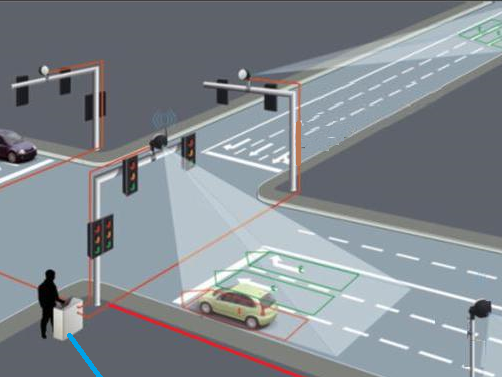
\includegraphics[width=(\textwidth / 4) * 3]{ObjectRecognitionSystemRepresentation.png}
            \caption{Sisteme bazate pe detectie de obiecte  
            (\href{https://english.mathrubhumi.com/news/kerala/knowing-traffic-camera-locations-isn-t-enough-to-escape-from-them-mvd-can-move-them-easily-1.7427787}{Sursa imagine} \textcopyright)}
            \label{fig:ObjectRecognitionSystem}
        \end{figure}

    \end{frame}

    \begin{frame}{Sisteme bazate pe senzori}
        O alta modalitate de a gestiona traficul este accea bazata pe senzori. 
        Aceasta presupune monitorizarea sosiri si plecari vehiculelor prin 
        intermediul datelor GPS.
        Astfel, am putea folosi tehnologia încorporată pentru a înregistra datele GPS și a le trimite
        la sistemul de monitorizare a traficului prin GSM/GPRS (Fig ~\ref{fig:SensorRecognitionSystem}). \\
        Dezavantajele acestei metode sunt faptul că implică costuri de implementare foarte mari, iar
        unele vehicule nu pot fi urmărite folosind sisteme de detectare radio.
        Această problemă poate fi abordata și cu ajutorul senzorilor de drum, dar ar necesita
        costuri chiar mai mari deoarece acestia ar trebui inlocuiti destul de des, 
        datorita uzuri parti carosabile si a constructiilor.
    \end{frame}

    \begin{frame}{Sisteme bazate pe senzori}
        \begin{figure}[h!]
            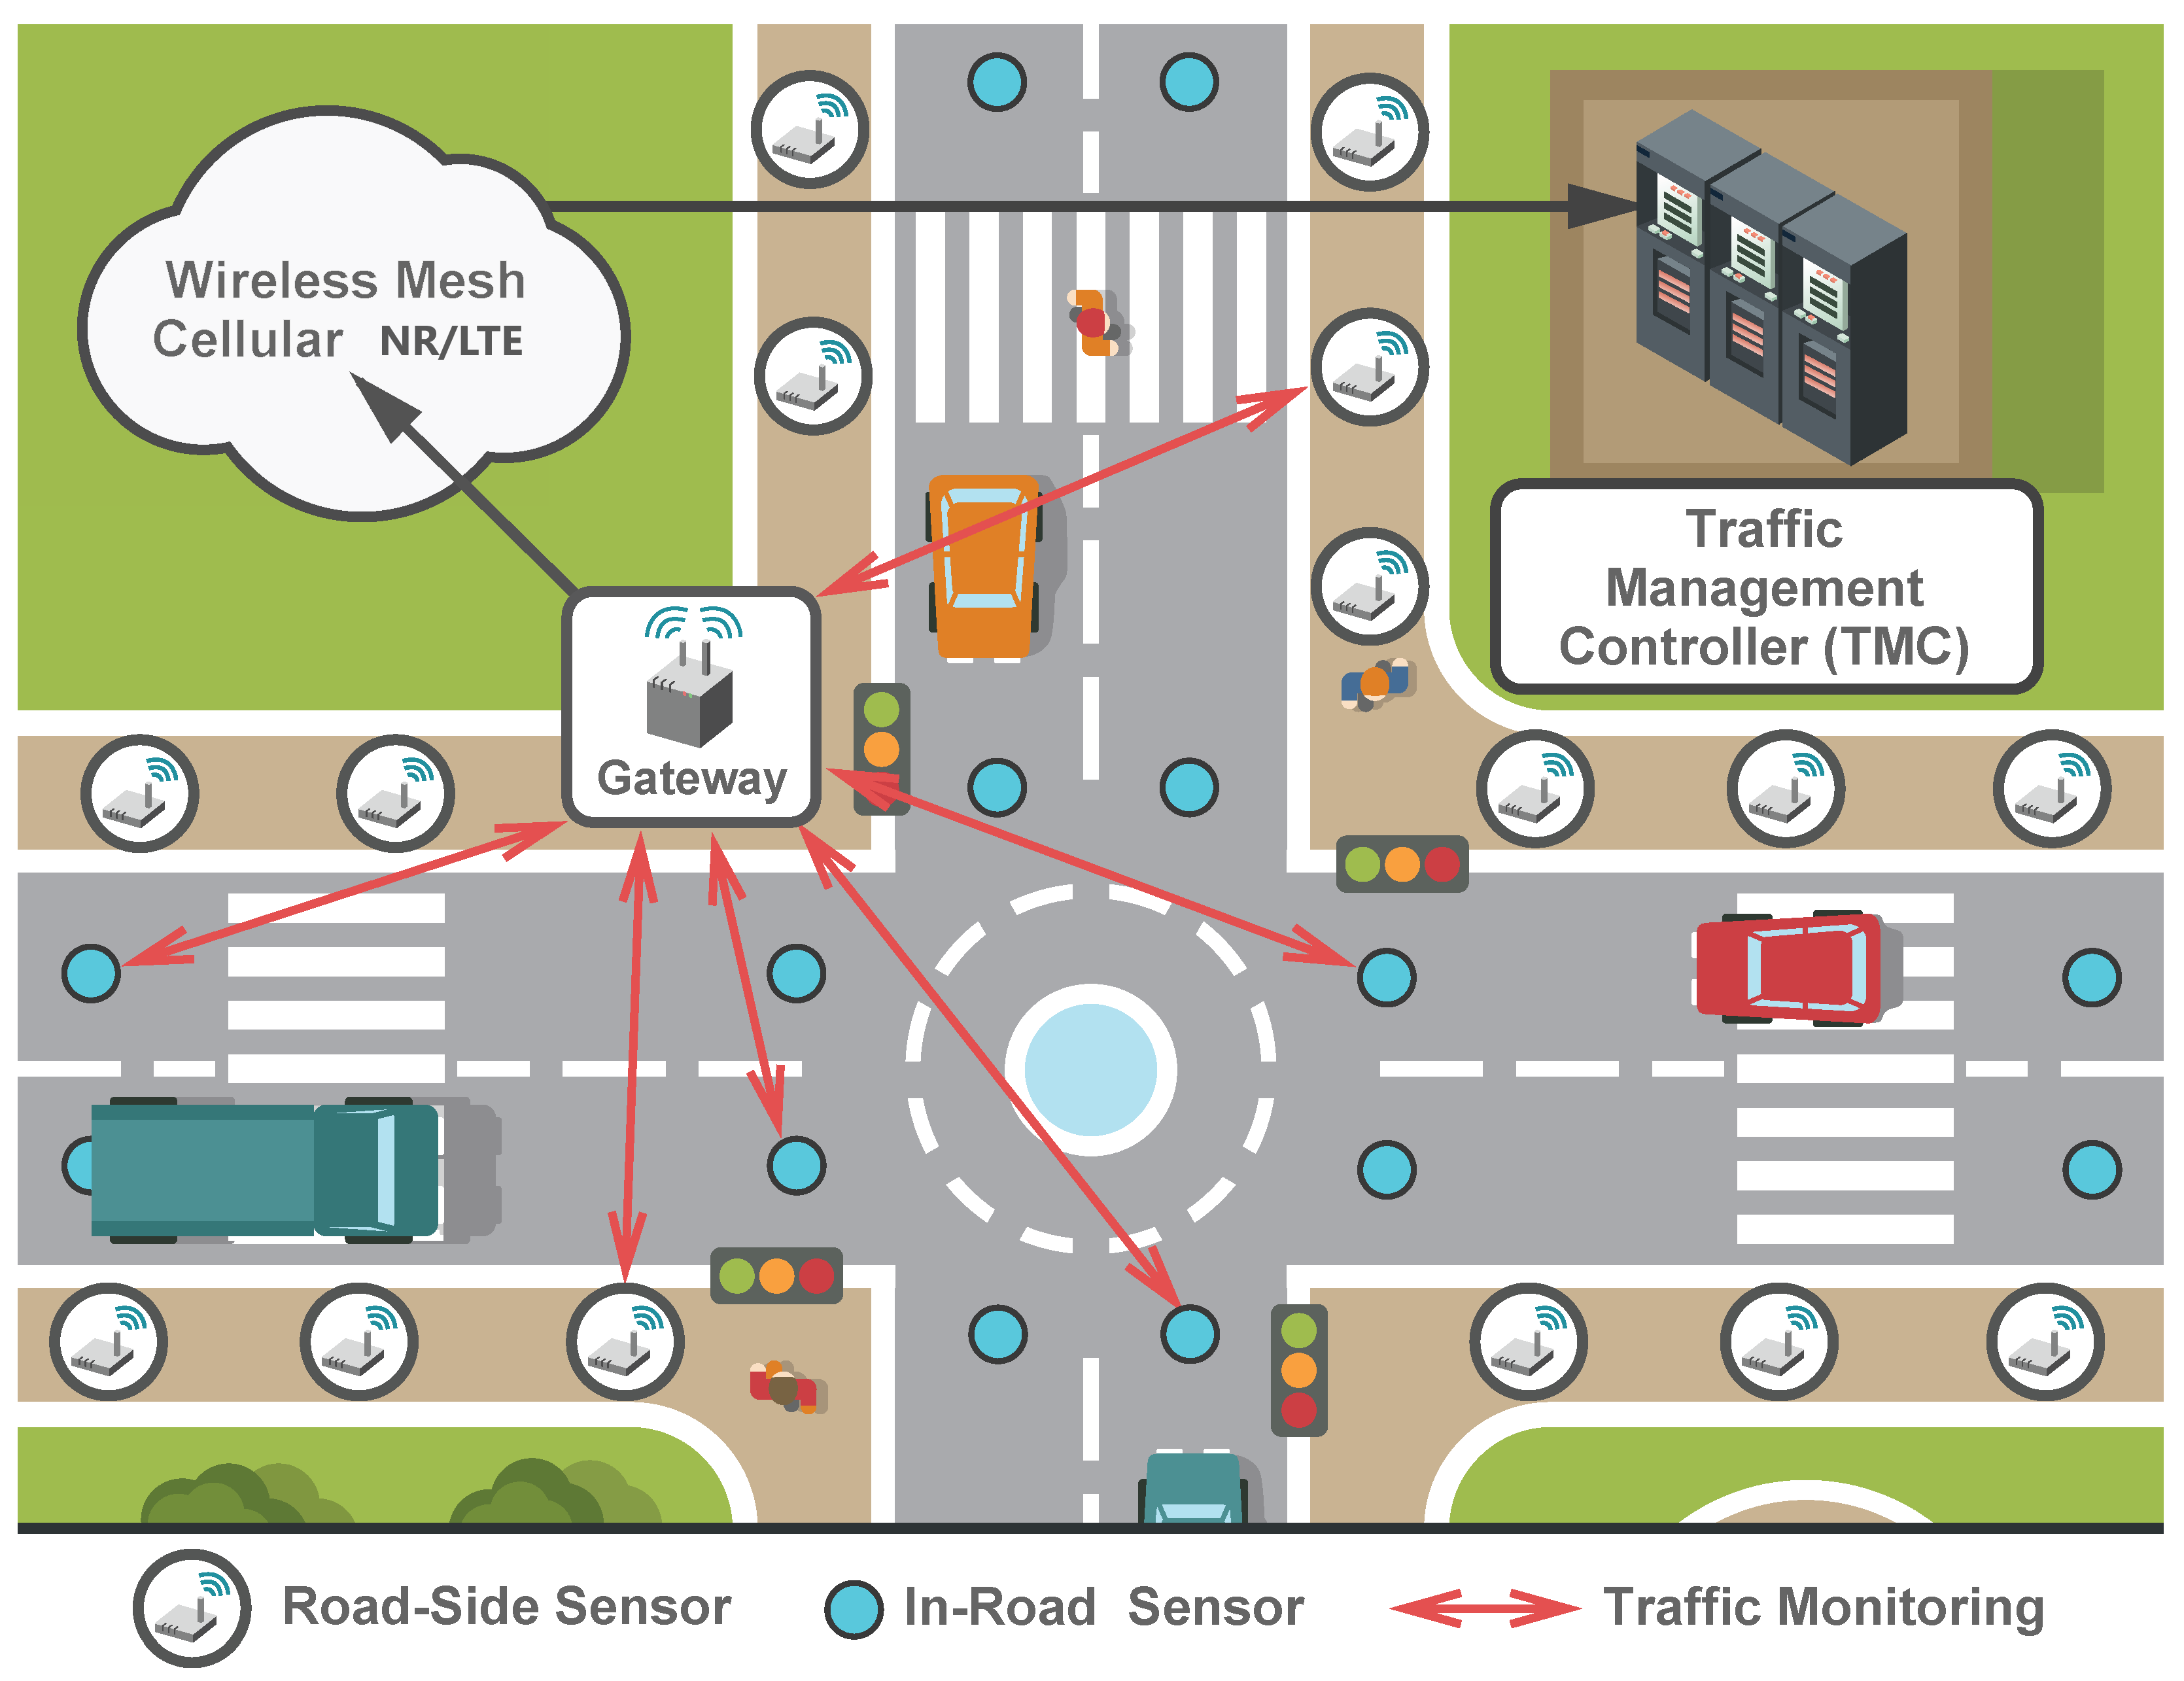
\includegraphics[width=(\textwidth / 4) * 3]{SensorsBasedTrafficControlSystemRepresentation.png}
            \caption{Sisteme bazate pe senzori 
            (\href{https://www.researchgate.net/figure/Communications-chain-of-data-feeds-in-smart-transportation_fig3_309740417}{Sursa imagine} \textcopyright)}
            \label{fig:SensorRecognitionSystem}
        \end{figure}
    \end{frame}

    \begin{frame}{Sisteme care sincronizeaza traficul}
        Sistemele de sincronizare a semafoarelor (TSC) urmăresc să minimizeze
        numărul de apariții STOP și GO prin adaptarea stari semafoarelor in intersectii.
        Această tehnică are ca si constrangere deplasarea la viteza constanta a vehiculelor,
        dand posibilitatea acestora sa treaca prin un lant de intersectii fara 
        oprire. La fel ca majoritatea altor sisteme, aceasta colecteaza 
        date despre traficul curent dar nu depinde de o anumita metoda specifica. 
        Cand vehiculele parcurg una dintre intersectii durata de verde creste, 
        la fel si cea de rosu pentru drumurile adiacente, dand posibilitatea curgeri 
        constante a traficului. \\
        Principalele dezavantaje ale acestei metode este ca in scenarii reale 
        conducatori nu vor respecta conditia de deplasare constanta in normele 
        legale de viteza, ducand la scenarii neprevazute, precum asteptarea 
        prelungita a rutelor secundare. De asemenea, metoda presupune prioritizarea 
        unei rute principale, in cazul in care doua sau mai multe rute principale 
        se intersecteaza traficul va fi desincronizat.

    \end{frame}

    \begin{frame}{Sisteme bazate pe logica fuzzy}
        Sistemele bazate pe logica fuzzy(FITS) au fost concepute initial 
        cu intentia de a imita un politist ce gestioneaza traficul dintr-o 
        intersectie. Acestea iau starea traficului si aplica reguli fuzzy 
        pentru a gestiona traficul. Astfel, starea traficului va fi 
        reprezentata de valori intra 0 si 1. De exemplu, durata timpului de 
        verde poate fi modelata pe baza setului fuzzy care include 4 stari:
        "none"(1), "scurt"(2), "moderat"(3), "lung"(4). \\
        In ciuda beneficiilor acestei abordari, asemnea altor algoritmi pe baza 
        de inteligenta artificiala, acesta necesita o perioada indelungata de 
        training, acesta facandu-se real-time datorita faptului ca traficul este 
        mult prea variadic si nu poate fi prezis. De asemenea, acest 
        training va trebui realizat pentru fiecare intersectie in parte, iar 
        rezultatele nu coincid intodeauna cu asteptarile, traficul putand 
        chiar fi ingreunat din cauza acestuia.
    \end{frame}

    \begin{frame}{Sisteme bazate pe logica fuzzy}
        \begin{equation}
            "none" - f(q) = max(min((10 - q) / 10, 2), 0)
        \end{equation}
        
        \begin{equation}
            "scurt" - f(q) = max(min(q / 10, (20 - q) / 10), 0)
        \end{equation}
        
        \begin{equation}
            "moderat" - f(q) = max(min(q / 5, (30 - q) / 5), 0)
        \end{equation}
        
        \begin{equation}
            "lung" - f(q) = max(min((50 - q) / 10, q / 2), 0)
        \end{equation}
    \end{frame}

    \begin{frame}{Sisteme bazate pe DSRC}
        DSRC sunt canale de comunicație fără fir unidirecționale sau
        bidirecționale special concepute pentru utilizare în automobile,
        care sunt utilizate în cea mai mare parte de către ITS pentru a
        comunica cu alte vehicule sau cu tehnologia infrastructurii.
        Acestea funcționează pe banda de 5,9 GHz a spectrului de frecvențe
        radio și sunt eficiente pe distanțe scurte si medii.
        Vitual Traffic Light(VTL) este o abordare inspirata din biologie 
        a controlului traficului care se bazeaza pe comunicare intre 
        vehicule (V2V) print utilizarea mesajelor DSRC.
        Ne putem imagina masinile ca fiind "routere in miscare", iar 
        intersectiile fiind "routere stationare". Ori de cate ori o 
        cale de transport este supraincarcata, una dintre rutele alternative 
        este blocata, astfel abordarea seamana mult cu tehnicile provenite 
        din retelistica.\\
        Principalul dezavantaj este faptul ca in momentul de fata sunt 
        multe vehicule care nu suporta acest tip de tehnologie. Astfel 
        infrastructura traficului nu permite lansarea sistemului.
    \end{frame}

    \begin{frame}{Sisteme bazate pe DSRC}
        \begin{figure}[h!]
            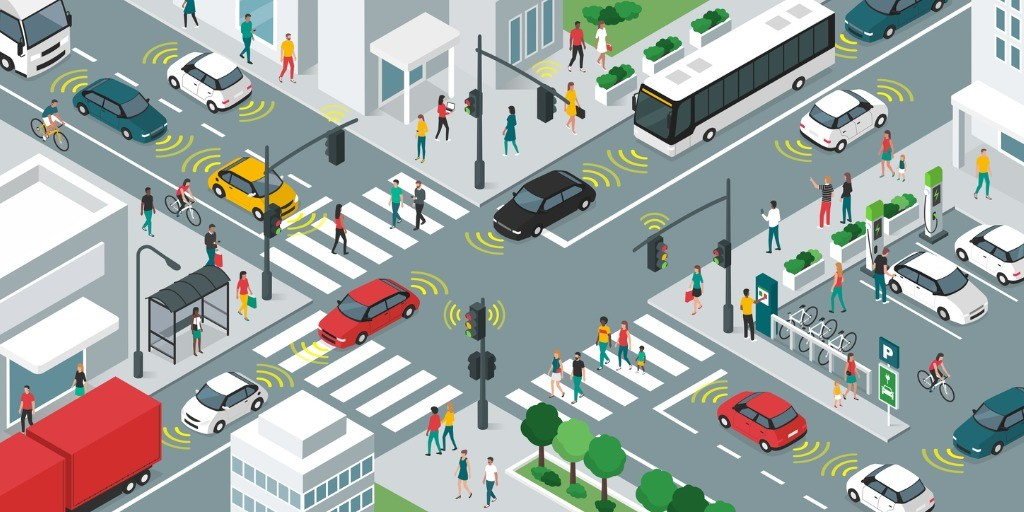
\includegraphics[width=\textwidth]{DSRCSystemModel.jpg}
            \caption{Sisteme bazate pe DSRC 
            (\href{https://www.frost.com/frost-perspectives/what-is-required-for-a-scalable-and-industry-wide-vehicle-to-everything-v2x-deployment/}{Sursa imagine} \textcopyright)}
            \label{fig:DSRCSystemModel}
        \end{figure}
        
    \end{frame}

\section{Motivatie, scopuri si obiective}
    \begin{frame}{Motivatie, scopuri si obiective}
        Ce ne-a determinat pe noi sa concepem acest nou tip de sistem este
        experienta in traficul din Timisoara, Romania. 
        Credem că sistemul de trafic de aici se bazează pe sisteme de sincronizare a semafoarelor,
        deoarece de cele mai multe ori, atunci când puteți prinde semaforul
        verde la un anumita intersecție, le veti prinde si pe restul ce urmeaza.
        Ce este problematic si credem ca este problema principala a soferilor 
        sunt orele de varf, cand traficul nu este gestionat bine si de 
        multe ori va trebuie sa astepti la acelasi semafor pana la 3 sau ba 
        chiar 4 cicluri de rosu si verde. Problema prezentata este datorita faptului 
        ca din cauza volumului mare de trafic, masinile nu vor mai putea circula 
        cu o viteza constanta iar traficul in sine va fi desincronizat.
        Acesta este doar un exemplu de trafic gestionat prost, dar 
        aceasta problema persista la nivel global, netinand cont de 
        tipul de sistem folosit, mereu vom ajunge la ambuteiaje. 
        Principalele noastre obiective sunt crearea unui sistem:

        \begin{itemize}[<+-| alert@+>]
            \item Performant si accesibil
            \item Adaptabil la orice conditie de trafic
            \item Scalabil la nivel global
            
        \end{itemize}

    \end{frame}

\section{O noua varianta flexibila si economica de a gestiona traficul}
    \begin{frame}{O noua varianta flexibila si economica de a gestiona traficul}
        Credem că viitorul gestionari traficului se va baza pe semnale
        asemanatoare cu cele DSRC. Deocamdată, infrastructura nu oferă o
        modalitate de a implementa acest tip de sisteme, asa ca am decis
        să dezvoltăm o nouă abordare care să combină și să preia cele mai
        bune caracteristici din toate tehnologiile descrise mai sus și să
        ofere o migrare ușoară. Pentru asta am conceput un sistem IPC 
        alcatuit din 2 tipuri de servere si 2 tipuri de clienti:
        \begin{itemize}[<+-| alert@+>]
            \item Servere: 
            \begin{enumerate}
                \item  Junction Main Server(JMS) - legat de intersectie si semafoare
                \item  Proxy - servere regionale ce asigura conectivitatea
            \end{enumerate}
            \item Clienti:
            \begin{enumerate}
                \item Traffic Observer(TO) - legat de catre o camera pe fiecare directie
                \item Vehicle Tracker(VT) - instalat direct pe autovehicul
            \end{enumerate}
        \end{itemize}

    \end{frame}

    \begin{frame}{Vehicle tracker}
        Clientul respectiv se va folosi de componentele deja instalate 
        pe o masina anume: GPS si Radio. Astfel acesta va determina 
        pozitia geografica atat cat si directia de mers si prin
        intermediul Proxy-ului se va conecta la urmatoarea intersectie, 
        semnaland intentia de traversare. Odata ce clientul respectiv 
        a trecut de intersectie, el se va deconecta si va interoga 
        ultimul proxy cunoscut. Astfel, vom avea o metoda rapida si 
        neperturbabila de a transmite date catre semafor, putand determina 
        usor starea traficului in orice momemnt.
    \end{frame}

    \begin{frame}{Proxy}
        Prima problema care trebuie rezolvata este cum anume se va 
        determina care este urmatoarea intersectie la care trebuie 
        sa se conecteze clientul. Pentru a rezolva aceasta dilema 
        am conceput un tip de server care actioneaza ca si un proxy. 
        El va fii amplasat la nivel regional si are rolul de a redirectiona 
        clienti instalati pe vehicule catre serverul instalat pe 
        intersectia corespunzatoare.
        Fiecare proxi are propriul sau set de date ce includ intersectiile 
        acoperite atat si o lista de noduri cu proxy-urile interconectate.
        Acest lucru ne permite scalarea sistemului pe orizontala, astfel 
        sistemul capatand posibilitatea de a fi lansat la nivel global 
    \end{frame}
    \begin{frame}{Traffic observer}
        Deoarece vrem ca sistemul nostru sa poata fi folosit inainte ca 
        o noua infrastructura pe baza de DSRC
        sa fie dezvoltata, am fost nevoiti sa adaugam o solutie alternativa 
        pentru determinarea starii traficului. Astfel am decis sa cream 
        un nou tip de client, ce se bazeaza pe detectia de obiecte, anume 
        un client ce poate detecta masinile. Acesta este amplasat pe 
        fiecare drum ce trece prin intersectie si necesita prezenta unei 
        camere. Odata instalat, el va actiona asemanator cu sistemele 
        bazate pe detectie de obiecte descrise mai sus. Acesta se poate 
        dezactiva oricand, avand ca si scop doar permiterea unei tranzitii 
        mai usoare catre sistemele DSRC odata ce avem infrastructura necesara.
    \end{frame}

    \begin{frame}{Junction main server}
        JMS sunt serverle principale, amplasate si legate direct la 
        semafoare ce au rolul de a gestiona traficul.
        
        În ceea ce privește algoritmul principal pentru managementul traficului,
        avem 8 faze ale traficului (Fig ~\ref{fig:Junction_phases}). 
        Scenariul cel mai simplu al traficului este acela in care cele 
        8 faze ale traficului vor fi parcurse intr-un mod circular pornind de
        la starea 1. Acest ciclu reprezinta modul in care se desfasoara 
        traficul in momentul de fata, dar noi vrem sa il depasim, sa putem sa sarim de la 
        o stare a traficului la alta "aleator" in orice moment.
        
    \end{frame}

    \begin{frame}{Junction main server}
        \begin{figure}[h!]
            \includegraphics[width=\textwidth]{Sketches/AvailableJunctionphases.png}
            \caption{Fazele traficului}
            \label{fig:Junction_phases}
        \end{figure}

    \end{frame}

    \begin{frame}{Junction main server}

        Pentru a determina urmatoare starea de trafic o sa avem cronometre asociate 
        fiecarei punct cardinal (E, W, N si S). In prima faza cronometrele vor fi 
        setate la o anumita valoarea, dar timpul de astepare va scadea dinamic, 
        odata cu aparitia vehiculelor. De asemena vom avea un timer asociat si 
        semnalului verde al semaforului. Odata ce acesta expira, ne vom calcula 
        urmatoarea stare a traficului. In caz ca niciun timer nu a expirat, vom 
        urma flow-ul normal al traficului, in caz contrar vom sari la starea corespunzatoare
        (Fig. ~\ref{fig:phasesSwitchingExample}). Putem insa avea si conflicte, de 
        exemplu nu putem lasa vehicule sa traverseze atat din N cat si din E. 
        Aceste scenarii le-am numit "scenarii de conflict" si dorim sa le 
        evitam pe cat posibil. In cazul nefericit al aparitiei unui astfel de 
        eveniment, am decis sa tratam scenariul folosind regula FIFO(Fig. ~\ref{fig:FaultyphaseSwitching}).
    
    \end{frame}

    \begin{frame}{Junction main server}
        \begin{figure}[h!]
            \includegraphics[width=\textwidth]{Sketches/SwitchingTroughphasesExample.png}
            \caption{Exemplu flow al traficului}
            \label{fig:phasesSwitchingExample}
        \end{figure}
        
    
    \end{frame}
    \begin{frame}{Junction main server}
        
        \begin{figure}[h!]
            \includegraphics[width=\textwidth]{Sketches/phaseSwitchingCaseToBeAvoided.png}
            \caption{Scenariu de conflict}
            \label{fig:FaultyphaseSwitching}
        \end{figure}

    \end{frame}

\section{Detalii de implementare}
    \begin{frame}{Detalii de implementare}
        Întregul sistem a fost dezvoltat folosind C++17, Python, Boost, OpenSSL, GLFW,
        MSVC WinAPI, OpenCV, Tensorflow, YoloV8 și MySQL. Sistemul în sine este
        tratat ca un proiect mare și împărțit în mai multe submodule: 

    \begin{itemize}
        \item librari
        \begin{itemize}
            \item Common
            \item CarDetector
            \item IPC
            \item GUIGLFW
        \end{itemize}
        
        \item executabile
        \begin{itemize}
            \item servere
            \begin{itemize}
                \item Proxy
                \item JunctionMainServer
                \item ObjectDetectionServer
            \end{itemize}
            \item  clienti
            \begin{itemize}
                \item VehicleTracker
                \item TrafficObserver
            \end{itemize}
            \item mediu de testare
        \end{itemize}
    \end{itemize}
    \end{frame}

    \begin{frame}{Common}
        Ideea principală a submodulului Common este să acționeze ca o
        bibliotecă ajutatoare. Oferă soluții la următoarele
        probleme frecvent întâlnite precum:
        \begin{itemize}
            \item Probleme de concurenta
            \item Parsarea datele produse de GPS 
            \item Interactiuni cu baza de date
            \item Parsarea fisierelor de configurare
            \item Crearea unor actiuni planificate
            \item Logarea sincrona in scenarii multifir de executie
        \end{itemize}
    \end{frame}

    \begin{frame}{IPC}
        Pentru a stabili comunicarea între toate executabilele, un sistem IPC nou
        a fost dezvoltat, ce se foloseste de Boost Asio pentru operatiile cu socket-uri.
        Logica în sine rulează pe 4 fire de executie: unul pentru menținerea contextului
        în funcțiune, unul pentru citire, unul pentru scriere și unul
        pentru notificarea progresului. \\
        Clientul are 4 metode principale, toate fiind rulate sincron:
        "connect", "disconnect", "send", "waitForAnswear". De fiecare dată când a
        se stabilește o nouă conexiune cu serverul, un nou obiect "Connexion"
        va fi creat care va fi responsabil de citire, scriere
        și furnizarea de mesaje.\\
        "Connexion" este responsabilă pentru citirea și scrierea mesajelor.
        Acționează ca un punct de mijloc între client și server. Aceasta
        are ca si obiect partajat o coadă de mesaje primite, astfel
        încât să poată notifica proprietarul că a sosit un nou mesaj. \\
    \end{frame}
    \begin{frame}{IPC}

        Serverul rulează pe 2 fire de execuție, unul pentru gestionarea
        operațiilor boost asio și unul pentru procesarea mesajelor primite.
        Are o listă de clienți deja conectați, iar conexiunea în sine este
        singura operație care este efectuată în mod asincron. Are 3 metode
        principale care pot fi suprascrise și care definesc comportamentul
        efectiv al serverului: "onClientConnect", "onClientDisconnect" și
        "onMessage", care sunt callback-uri către evenimente IPC
        . Dacă, de exemplu, un integrator ar dori să utilizeze framework-ul
        nostru IPC, tot ce ar trebui să facă ar fi să suprascrie aceste
        callback-uri furnizate.\\

        Pentru a defini structura mesajelor, am creat și o clasă
        specifica. Antetul mesajului conține dimensiunea acestuia,
        dacă are prioritate (este de la un vehicul de urgență) și tipul
        mesajului care este trimis, precum și un ID. Datele salvate în
        corpul mesajului sunt în format de octeți iar adaugarea/extragerea de date 
        functioneaza ca si o stiva.
    \end{frame}

    \begin{frame}{GUIGLFW}
        Pentru a putea vizualiza datele reale, am creat un modul GUI.
        Acesta este doar în scopuri de demonstrație/testare și poate fi
        dezactivat folosind un flag. Pentru a realiza acest lucru, am
        utilizat GLFW, mai exact am pre-desenat intersecția și am
        legat-o de cronometrele intersectiei. În ceea ce privește
        mașinile, am avut o coadă de acțiuni în așteptare și ori de
        câte ori o mașină era detectată de JMS, acțiunea de desenare era
        pusă în coadă. Acțiunea în sine poate de asemenea adauga la randul 
        ei o alta actiune, daca masina nu a depasit inca fereastra.
        Deoarece dorim ca scena să acționeze ca o intersecție,
        atunci când suntem pe punctul de a traversa intersecția în timpul
        desenării, am intarziat-o atat timp cat lumina rosie persista (Fig ~\ref{fig:GUI JMS}).
        
    \end{frame}

    \begin{frame}{GUIGLFW}
        \begin{figure}[h!]
            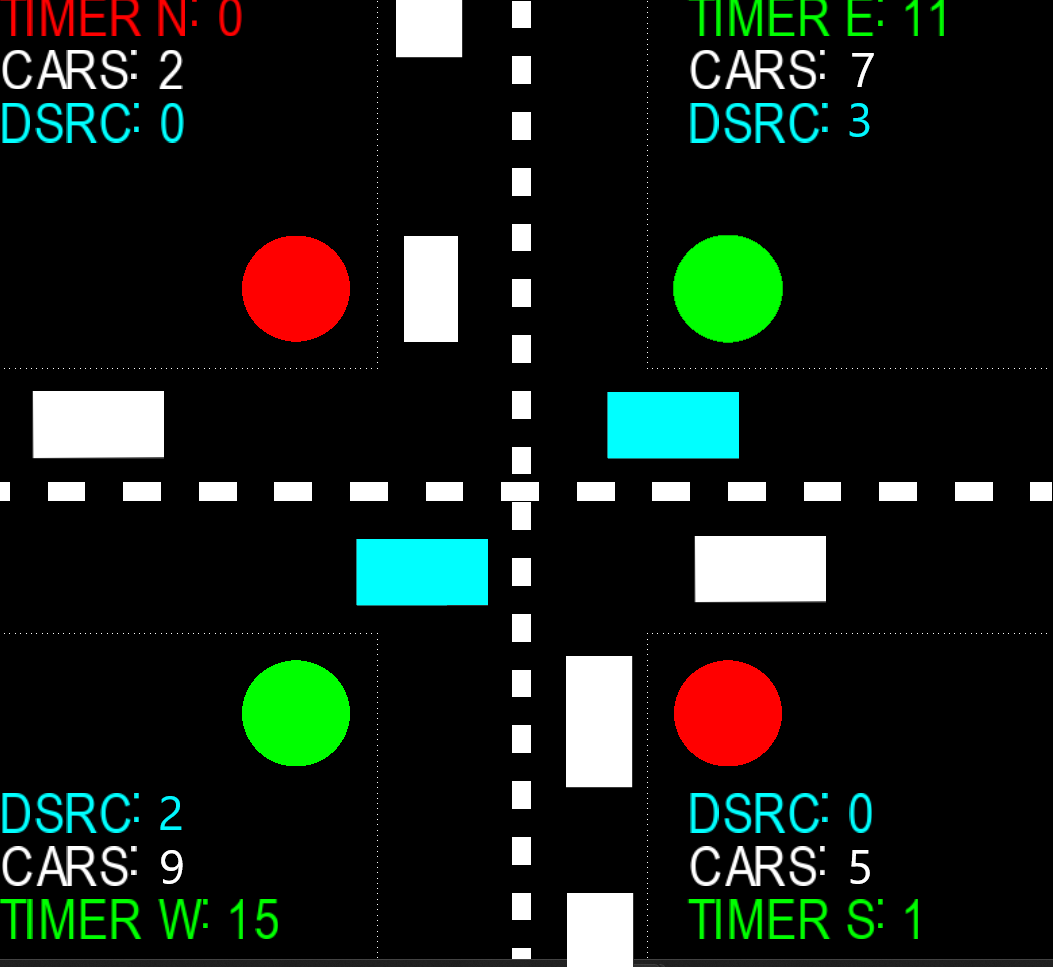
\includegraphics[width=(\textwidth / 3) * 2]{running/GUI_JMS.png}
            \caption{GUI JMS}
            \label{fig:GUI JMS}
        \end{figure}

    \end{frame}
    \begin{frame}{Car Detector}
        Pentru a putea conecta la camerele de trafic rutier și pentru a
        determina numărul de vehicule care intră/ies, am creat wrappere peste
        biblioteca OpenCV. Întregul proces funcționează în felul următor:
        începe prin detectarea obiectelor în mișcare într-un cadru dat,
        încearcă să prezică poziția lor următoare și odată ce acestea
        traversează linii imaginare, acestea sunt înregistrate dacă s-au
        dovedit a fi mașini. Pentru a îmbunătăți șansele de
        înregistrare efectivă a trecerii unei mașini, am considerat
        mașinile ca obiecte punctiforme, luând în considerare doar punctul
        central al dreptunghiului delimitator ca fiind mașini reale.
        Clasificarea mașinilor în sine nu este realizată de modulul dat
        datorită incompatibilității actuale dintre Tensorflow și
        OpenCV in C++, ci de către ObjectDetectionServer scris în Python.
        Modulul CarDetector acționează doar ca un client și trimite
        octeții reali ai imaginii decupate ce reprezinta obiecetele 
        in miscare către server și așteaptă un răspuns.
    \end{frame}

    \begin{frame}{Object Detection Server}
        Pentru a putea detecta dacă sunt prezente mașini, am încercat
        să utilizăm două arhitecturi diferite: una bazată pe YOLOv8 și
        una utilizând API-ul de detecție a obiectelor TensorFlow, în
        timp ce am folosit același set de date pentru antrenament.
        In urma unei analize indelungate, ce poate fi regasita in lucrare, 
        am determinat ca modelul antrenat folosind Tenserflow este mult 
        mai potrivit pentru scenariul nostru. Am folosit SSD MobileNet, un 
        tip de retea neuronala convolutionara ce a fost preantrenata si 
        este folosita deseori pe sisteme cu resurse limitate. Acuratetea medie 
        a modelului antrenat de noi este de 60\%, iar acesta este incarcat de 
        catre un server simplist scris in Python.
    \end{frame}

    \begin{frame}{Proxy}
        Proxy-ul este un wrapper peste implementarea serverului care
        asigură conexiunea între VT și JMS.
        Fiecare proxy este conectat la propria sa bază de date,
        care conține o listă de intersecții, proxy-uri și zona acoperită
        de acestea. Modul de funcționare este destul de simplu: dacă un
        client interoghează proxy-ul pentru următoarea intersecție,
        acesta caută în baza de date. Dacă găsește o intersecție
        potrivită, trimite datele de conexiune, în caz contrar
        redirecționează vehiculul către proxy-ul cel mai apropiat.
        Acest proces se repetă până când ajunge în cele din urmă la o
        intersecție validă sau mașina iese din zona de acoperire
        (de exemplu, dacă mașina se află undeva pe o navă în mijlocul
        mării, nu există niciun motiv să o conectăm la o intersecție).
    \end{frame}
    \begin{frame}{Proxy}
        \begin{figure}[h!]
            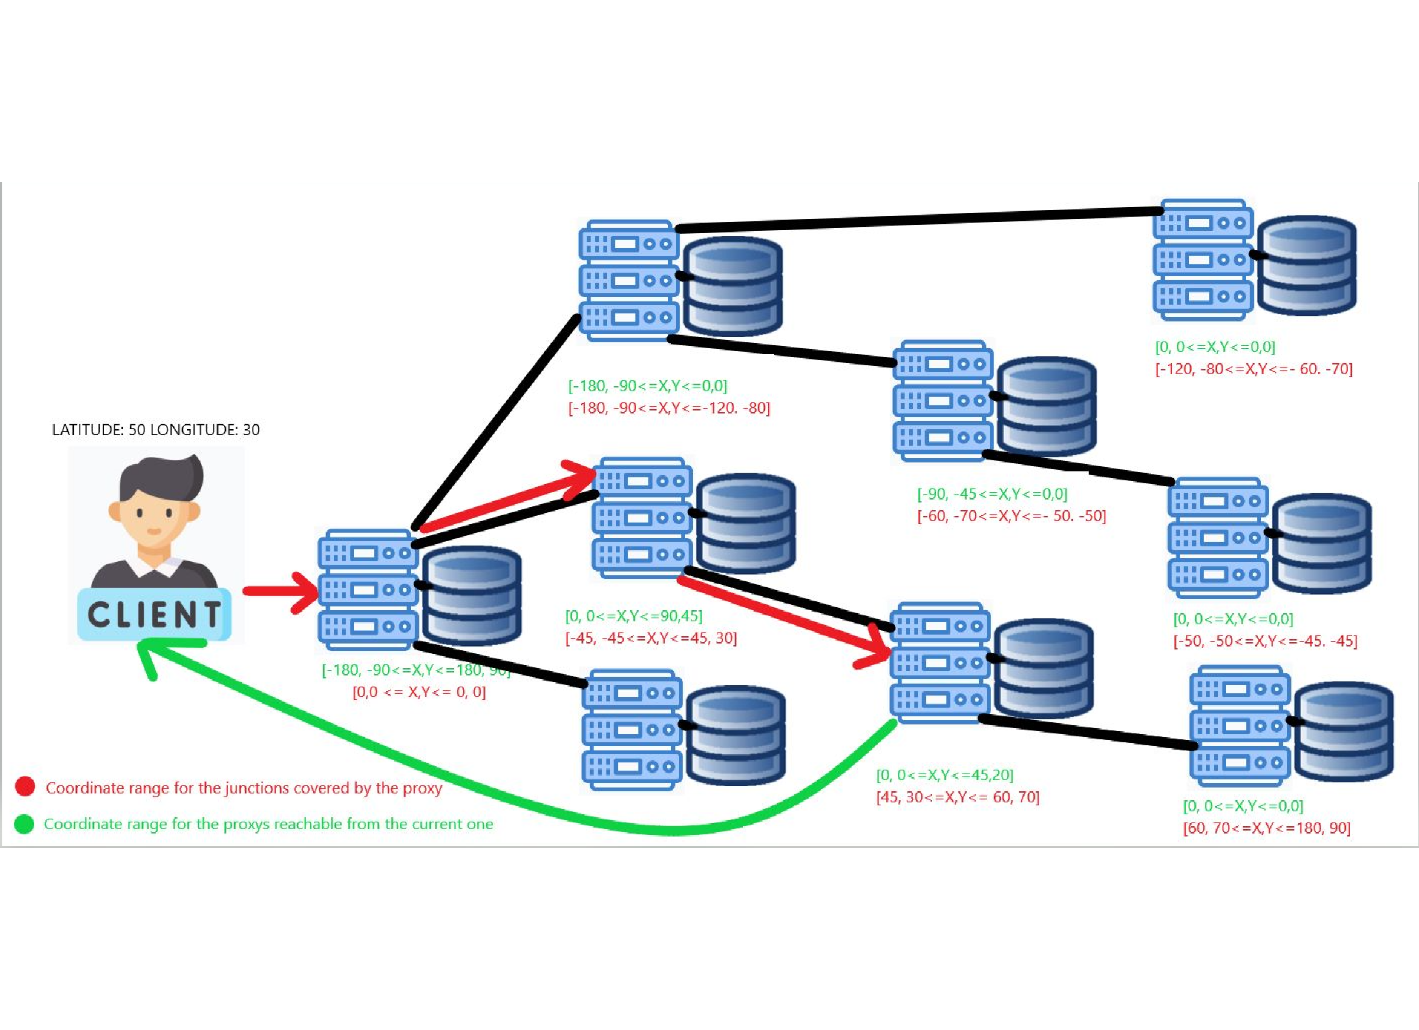
\includegraphics[width=(\textwidth / 6) * 5]{Sketches/ProxyFlowV2.png}
            \caption{Flow-ul de interogare a proxy-urilor}
            \label{fig:Proxy querys flow}
        \end{figure}
    \end{frame}


    \begin{frame}{JunctionMainServer}
        Executabilul este un wrapper peste implementarea serverului si 
        gestionează stările traficului. Acesta urmărește vehiculele
        care urmeaza sa treaca prin intersectie și cronometrează fiecare stare de trafic.
        Implementarea în sine este concepută ca un state machine, 
        în care stările sunt reprezentate de stările traficului,
        iar evenimentele sunt reprezentate de expirarea cronometrelor.
        Fiecare stare are asociat un cronometru care scade în mod
        normal sau când este detectat un vehicul care urmeaza sa treaca
        prin intersectie. Ori de câte ori ne aflăm într-o anumită stare,
        cronometrul corespunzător este oprit și apoi resetat, iar 
        durata acestuia este recalculata in functie de trafic.
        Modul in care update-ul cronometrelor influenteaza traficul se
        poate vedea in figura ~\ref{fig:Timer Increase/Decrease Impact}
    \end{frame}

    \begin{frame}{JunctionMainServer}
        \begin{figure}[h!]
            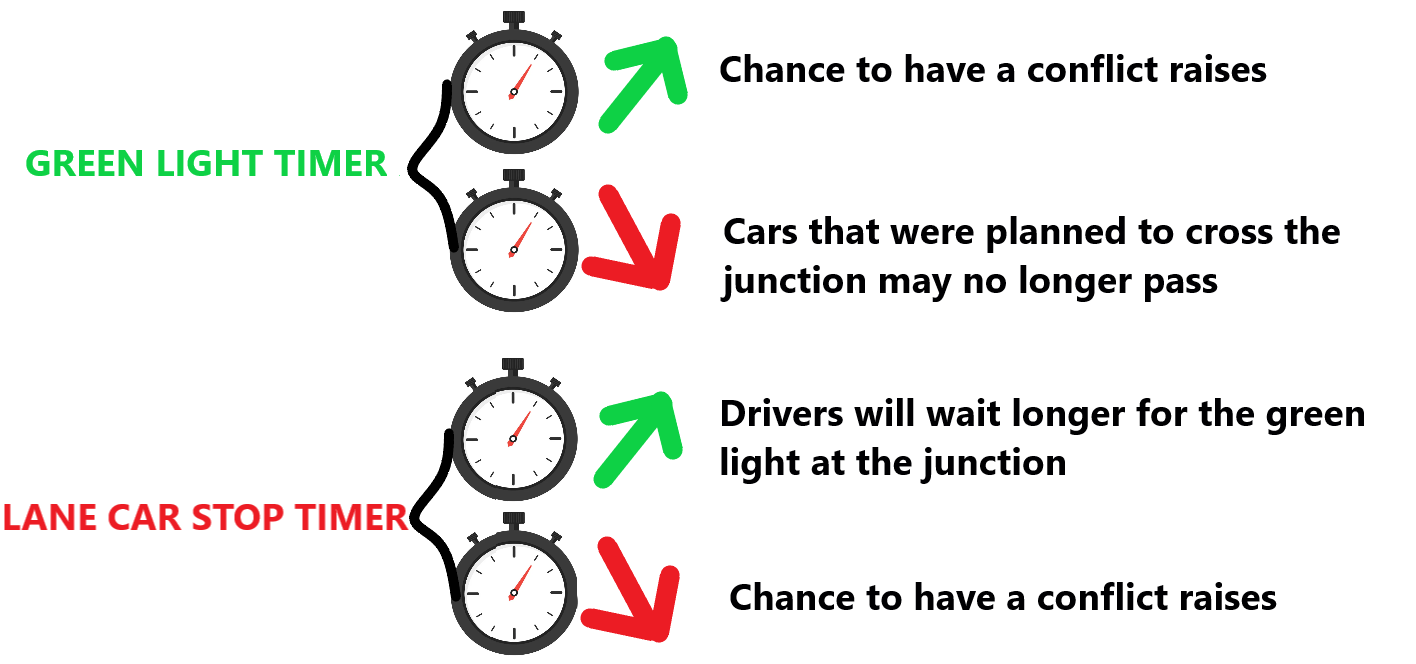
\includegraphics[width=\textwidth]{Sketches/TimerIncreaseDecreaseImpact.png}
            \caption{Impactul cresteri/scaderi durati cronometrului}
            \label{fig:Timer Increase/Decrease Impact}
        \end{figure}
    \end{frame}

    \begin{frame}{JunctionMainServer}
        Principiul de baza pe care incercam sa il obtinem este un timp 
        minim de astepare fara a intra in stari de conflict. Pentru 
        acest lucrur am retinut o medie a vehiculelor ce au trecut 
        de intersectie in timpul lumini verzi a semaforului si daca 
        suntem sau nu in stare de conflict. Din cauza complexitati 
        ridicate a algoritmilor de detectie a obiectelor, pentru a 
        numara vehiculele ce au trecut de semafor, ne vom baza doar 
        pe mesajele primite de la VTs. Astfel avem 4 scenarii 
        posibile iar modul de tratare se poate vedea in figura ~\ref{fig:Faulty Scenarios Handling}
    \end{frame}

    \begin{frame}{JunctionMainServer}    
        \begin{figure}[h!]
            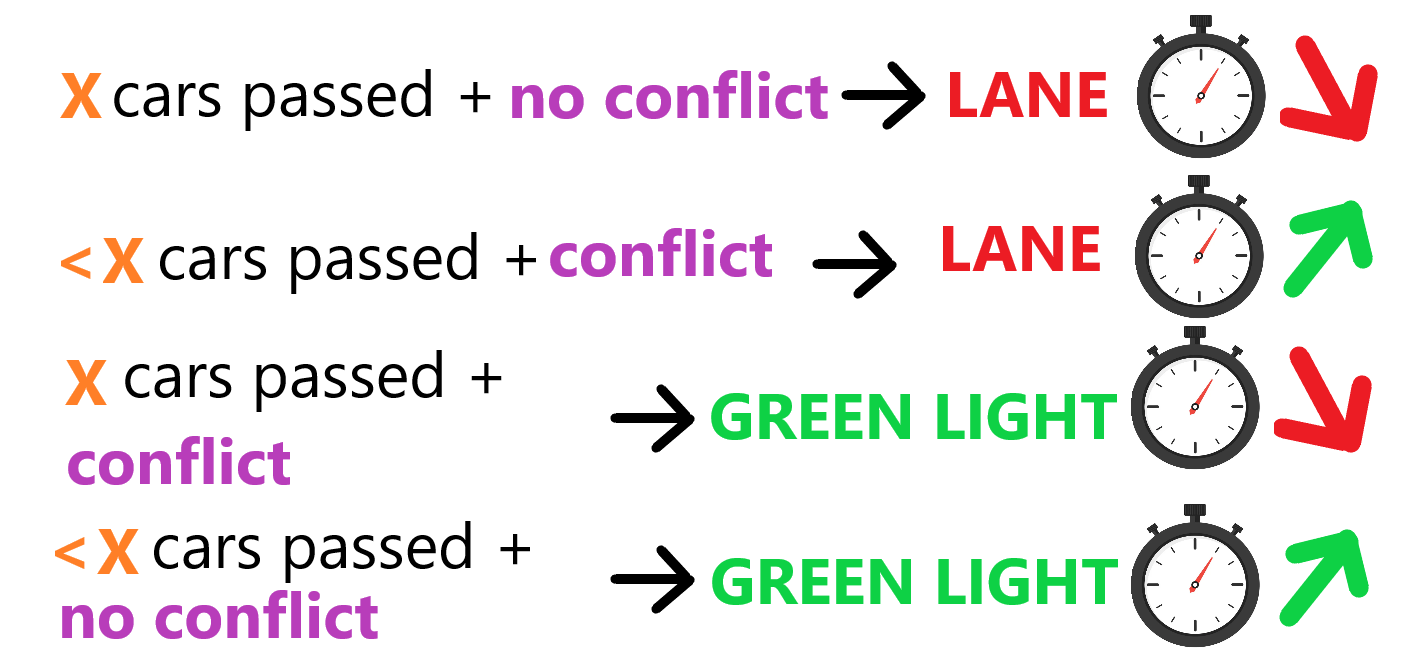
\includegraphics[width=\textwidth]{Sketches/FaultyScenariosHandling.png}
            \caption{Faulty Scenarios Handling}
            \label{fig:Faulty Scenarios Handling}
        \end{figure}
    \end{frame}

    \begin{frame}{TrafficObserver}
        Executabilul este un wrapper peste client ce incarca functionalitatile modulului de 
        detectie de masini (Fig ~\ref{fig:Running client samples}) si trimite periodic mesaje la server.
        De asemenea, din cauza volumului mare de mesaje trimise si potentialelor exploit-uri, 
        am adaugat o parola de conectare la server si un schimb de chei publice, pentru 
        a impiedica eventualele atacuri cibernetice.
        \begin{figure}[h!]
            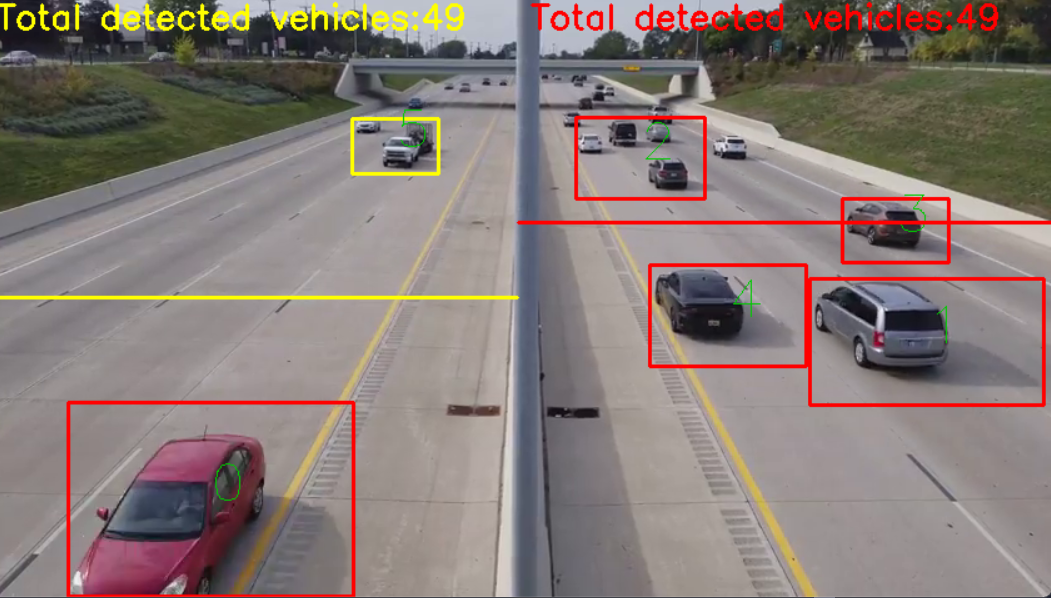
\includegraphics[width=(\textwidth / 3) * 2]{TrafficDetectionRunningExample2.png}
            \caption{Exemplu detectie masini }
            \label{fig:Running client samples}
        \end{figure}

        
    \end{frame}

    \begin{frame}{VehicleTracker}
        Executabilul este un wrapper peste client. La pornire acesta 
        incepe sa parseze datele geografice dintr-un stream de date
        (in momentul testari dintr-un fisier). Astfel, din formatul NMEA
        al datelor, anume din mesajele de tip GPGLL, GPGGA si GPRM se extrag 
        coordonatele geografice curente. Pentru a afla de asemnea directia 
        acesta citeste doua coordonate geografice distincte consecutive si determina 
        aproximativ directia predominanta. De exemplu daca vehiculul merge spre 
        NE dar acesta se deplaseaza mai mult spre N, directia acestuia va fi N.
        Odata ce am obtinut coordonatele geografice cat si directia, acestea 
        vor fi trimise la proxi pentru a determina urmatoare intersectie. 
        Clientul se va conecta la server-ul corespunzator, va astepta 
        pana cand acesta va trece de intersectie si va relua procesul de la capat.
    \end{frame}

    \begin{frame}{Mediu de testare}
        
        Pentru a putea testa întregul nostru sistem, am creat un
        executabil care să emuleze condițiile de trafic și să ruleze
        sistemul nostru. Executabilul primește mai multe fișiere de
        configurare ca intrare și poate rula simultan mai multe servere
        (JMS/Proxy-uri) și mai mulți clienți de orice tip, in orice fel 
        de combinatie. Pentru a emula mișcarea
        clienților instalati pe vehicule, am generat date GPS cu ajutorul
        \href{https://www.nmeagen.org/}{NMEAGEN}, iar pentru a simula
        inputul camerelor am colectat mai multe videoclipuri.
    \end{frame}

\section{Concluzii, defecte ale sistemului si directii viitoare}
    \begin{frame}{Concluzii, defecte ale sistemului si directii viitoare}
        În această teză, prin analiza cercetărilor existente,
        exemplelor de implementare și tendințelor emergente, am obținut
        idei valoroase cu privire la eficacitatea și potențialul
        sistemelor de gestionare a traficului. Cu datele colectate,
        am oferit o nouă modalitate alternativă de gestionare a traficului
        prin definirea și implementarea unui nou sistem de trafic,
        pe care credem că va îmbunătăți semnificativ fluxul de trafic. Acesta 
        se poate adapta la conditiile de trafic, poate fi lansat la nivel global si 
        reprezinta o punte de trecere catre sistemele DSRC. De asemnea acesta 
        este accesibil deoarece nu necesita prezenta tuturor componentelor 
        hardware si/sau software pentru o buna functionare, iar majoritatea 
        cerintelor sunt deja indeplinite.
    \end{frame}

    \begin{frame}{Concluzii, defecte ale sistemului si directii viitoare}
        Unul din principalele defecte ale sistemului este faptul ca 
        exista inca scenarii de exploit in sistem.
        Ca si imbunatatire, trebuie stabilita o limita maxima de incercari de 
        conectare, atat si creat un "blacklist" pentru IP-urile userilor maliciosi. \\
        De asemenea se poate integra un algoritm care aproximeaza zonele ocupate ale 
        carosabilului, dar asta ar presupune o complexitate destul de ridicata si o 
        ingreunare a sistemului, fiind discutabil daca se merita sau nu acest 
        tradeoff de performanta pentru o mai buna securitate.\\
        Un alt defect care se poate observa, este faptul ca, ca si orice alt 
        sistem bazat pe detectie de obiecte, conditiile meteo ii vor 
        afecta performanta. Ca si rezolvare la aceasta problema, se poate 
        incerca detectia de obiecte pe baza altor tipuri de imagini, mai putin 
        perturbabile de meteo, cum ar fi imaginile radio care au dovedit a fi 
        un suport mai bun de antrenare a modelului, cel putin in conditii de ceata.
        O ultima imbunatatire ce ar trebui adusa asupra sistemului este crearea unui 
        model nou specializat doar pe detectia de masini.
    \end{frame}

\end{document}